
As shown in Section~\ref{sec:ExpectedSig} we expect to see significant improvements in the limits for 
particles that decay to gluon-gluon and possible improvements in searches that involve a quark-gluon 
final state. In both cases the optimal search is by selecting only on the gluon initiated jets with a 
nominal efficiency of 75\%.  

The choice of operating point will be confirmed by using pseudo-data to test 
the selection efficiency by 
running the fitting and limit setting procedure of samples generated with selection efficiencies ranging from 
65 to 90\% in 5\% steps. 

\subsection{Signals that decay to gluon-gluon.}


The pseudo-data tests of the significance of gluon-gluon searches are studied using  \Hprime\ models as the signal. 
Each pseudo-data sample is fitted with SWiFt to estimate the background and then passed through \texttt{HistFitter}. 
For the initial estimation of the effectiveness of the selection we only include statistical uncertainties, 
the uncertainty on the integrated luminosity and an additional uniform 5\% uncertainty that is an initial 
guess of the magnitude of the uncertainty due to the gluon selection.  These results are compared to limits 
produced using pseudo-data created assuming no gluon selection has been applied. 

The resulting expected limits are plotted in Fig.~\ref{fig:GluonSignalSignificancePD}  and show a clear 
improvement in the expected limits for all the investigated gluon selection criteria. If we take the 
ratio of the expected cross section limits with gluon selection applied divided by the limits with no 
selection applied (Fig.~\ref{fig:GluonSignalSignificanceRatio}) shows that there is no obvious optimal
selection criteria. We have chosen 75\% as it performs well at masses above 4\,\TeV\ while we finalise 
the estimation of systematic uncertainties. 


\begin{figure}[htb]
 \centering
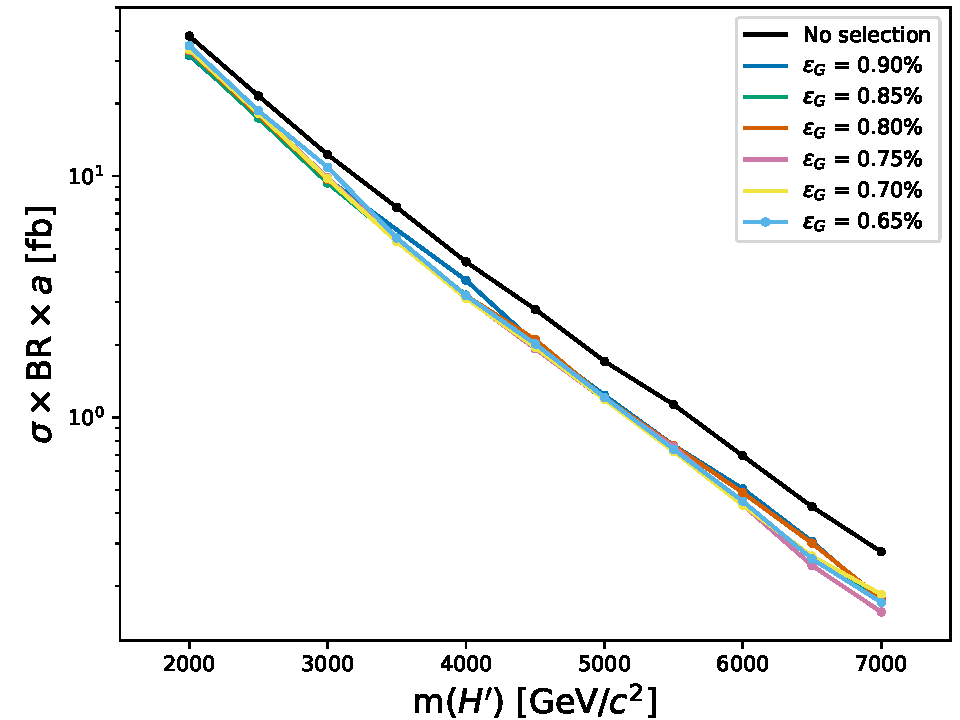
\includegraphics[width=0.75\textwidth]{figures/significance/Limits_GG_All.pdf}
\caption{ The expected cross section limits for a \Hprime\ with masses from 2000 to 7000\,\GeV\ 
for $\epsilon_{gG}$ ranging from 65 to 90\% compared to the significance calculated with 
   no gluon selection applied.
  \label{fig:GluonSignalSignificancePD}}
\end{figure}

\begin{figure}[htb]
 \centering
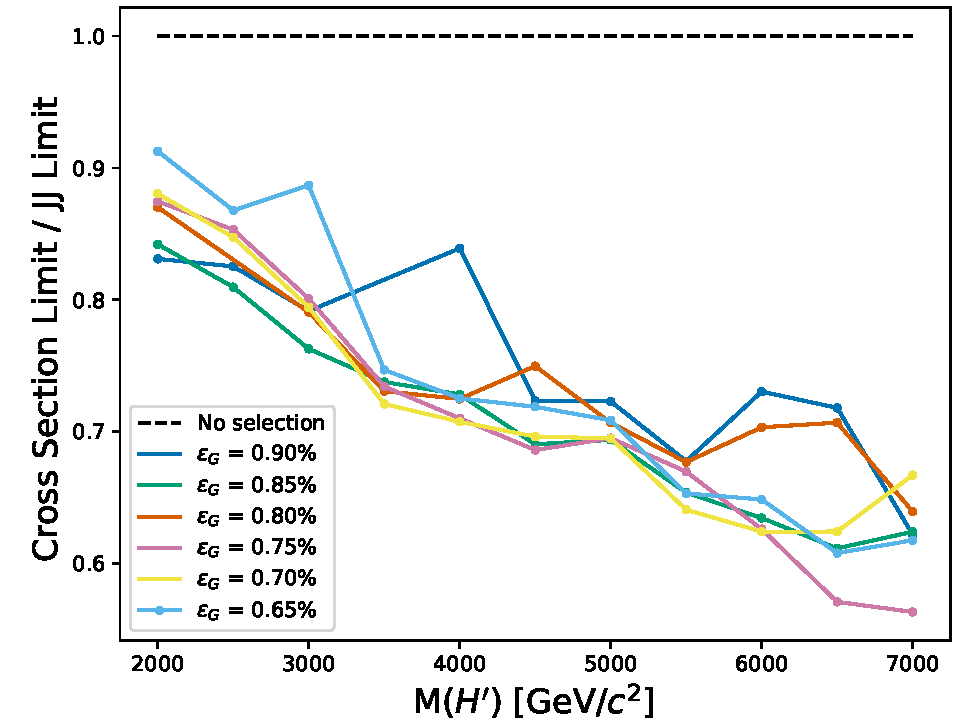
\includegraphics[width=0.75\textwidth]{figures/significance/Ratio_GG_All.pdf}
\caption{ The ratio of the expected cross section limits with gluon selection applied divided by the limits with no selection applied for a \Hprime\ with masses from 2000 to 7000\,\GeV. \label{fig:GluonSignalSignificanceRatio}}
\end{figure}


\subsection{Signals that decay to quark-gluon.}

The same procedure is applied for the significance of quark-gluon searches except that a \qstar\ is used for the signal. 
The resulting expected limits are plotted in Fig.~\ref{fig:QuarkGluonSignalSignificancePD}  and show a small 
improvement in the expected limits for all the investigated gluon selection criteria. If we take the 
ratio of the expected cross section limits with gluon selection applied divided by the limits with no 
selection applied (Fig.~\ref{fig:QuarkGluonSignalSignificanceRatio}) shows that there is no obvious optimal
selection criteria. We have chosen 75\% as it performs well at masses above 4\,\TeV\ while we finalise 
the estimation of systematic uncertainties. 



\begin{figure}[htb]
 \centering
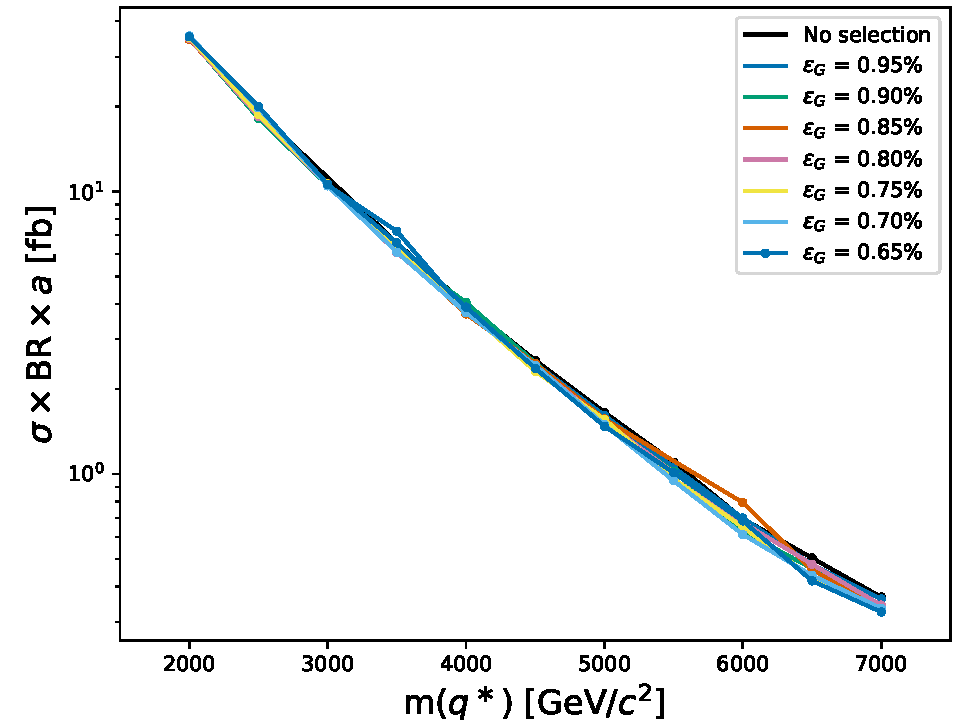
\includegraphics[width=0.75\textwidth]{figures/significance/Limits_QG_All.pdf}
\caption{ The expected cross section limits for a \qstar\ with masses from 2000 to 7000\,\GeV\ 
for $\epsilon_{gG}$ ranging from 65 to 90\% compared to the significance calculated with 
   no gluon selection applied.
  \label{fig:QuarkGluonSignalSignificancePD}}
\end{figure}

\begin{figure}[htb]
 \centering
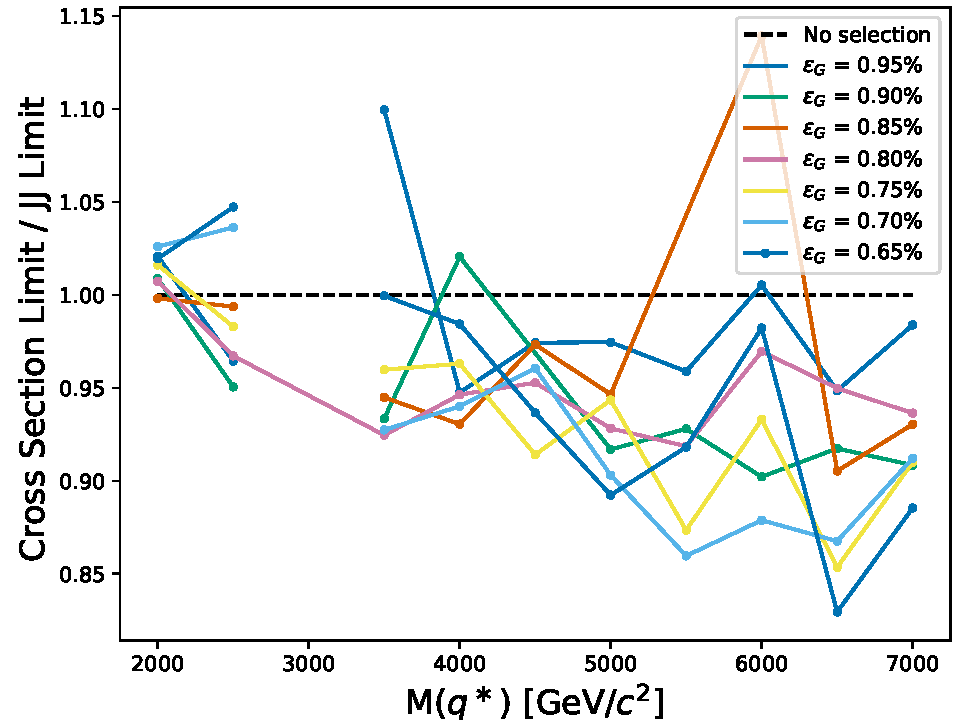
\includegraphics[width=0.75\textwidth]{figures/significance/Ratio_QG_All.pdf}
\caption{ The ratio of the expected cross section limits with gluon selection applied divided by the limits with no selection applied for a \qstar\ with masses from 2000 to 7000\,\GeV. \label{fig:QuarkGluonSignalSignificanceRatio}}
\end{figure}


%Ratio_GG_All.pdf


%\begin{figure}[p]
% \centering
%
% \subfigure[JJ] {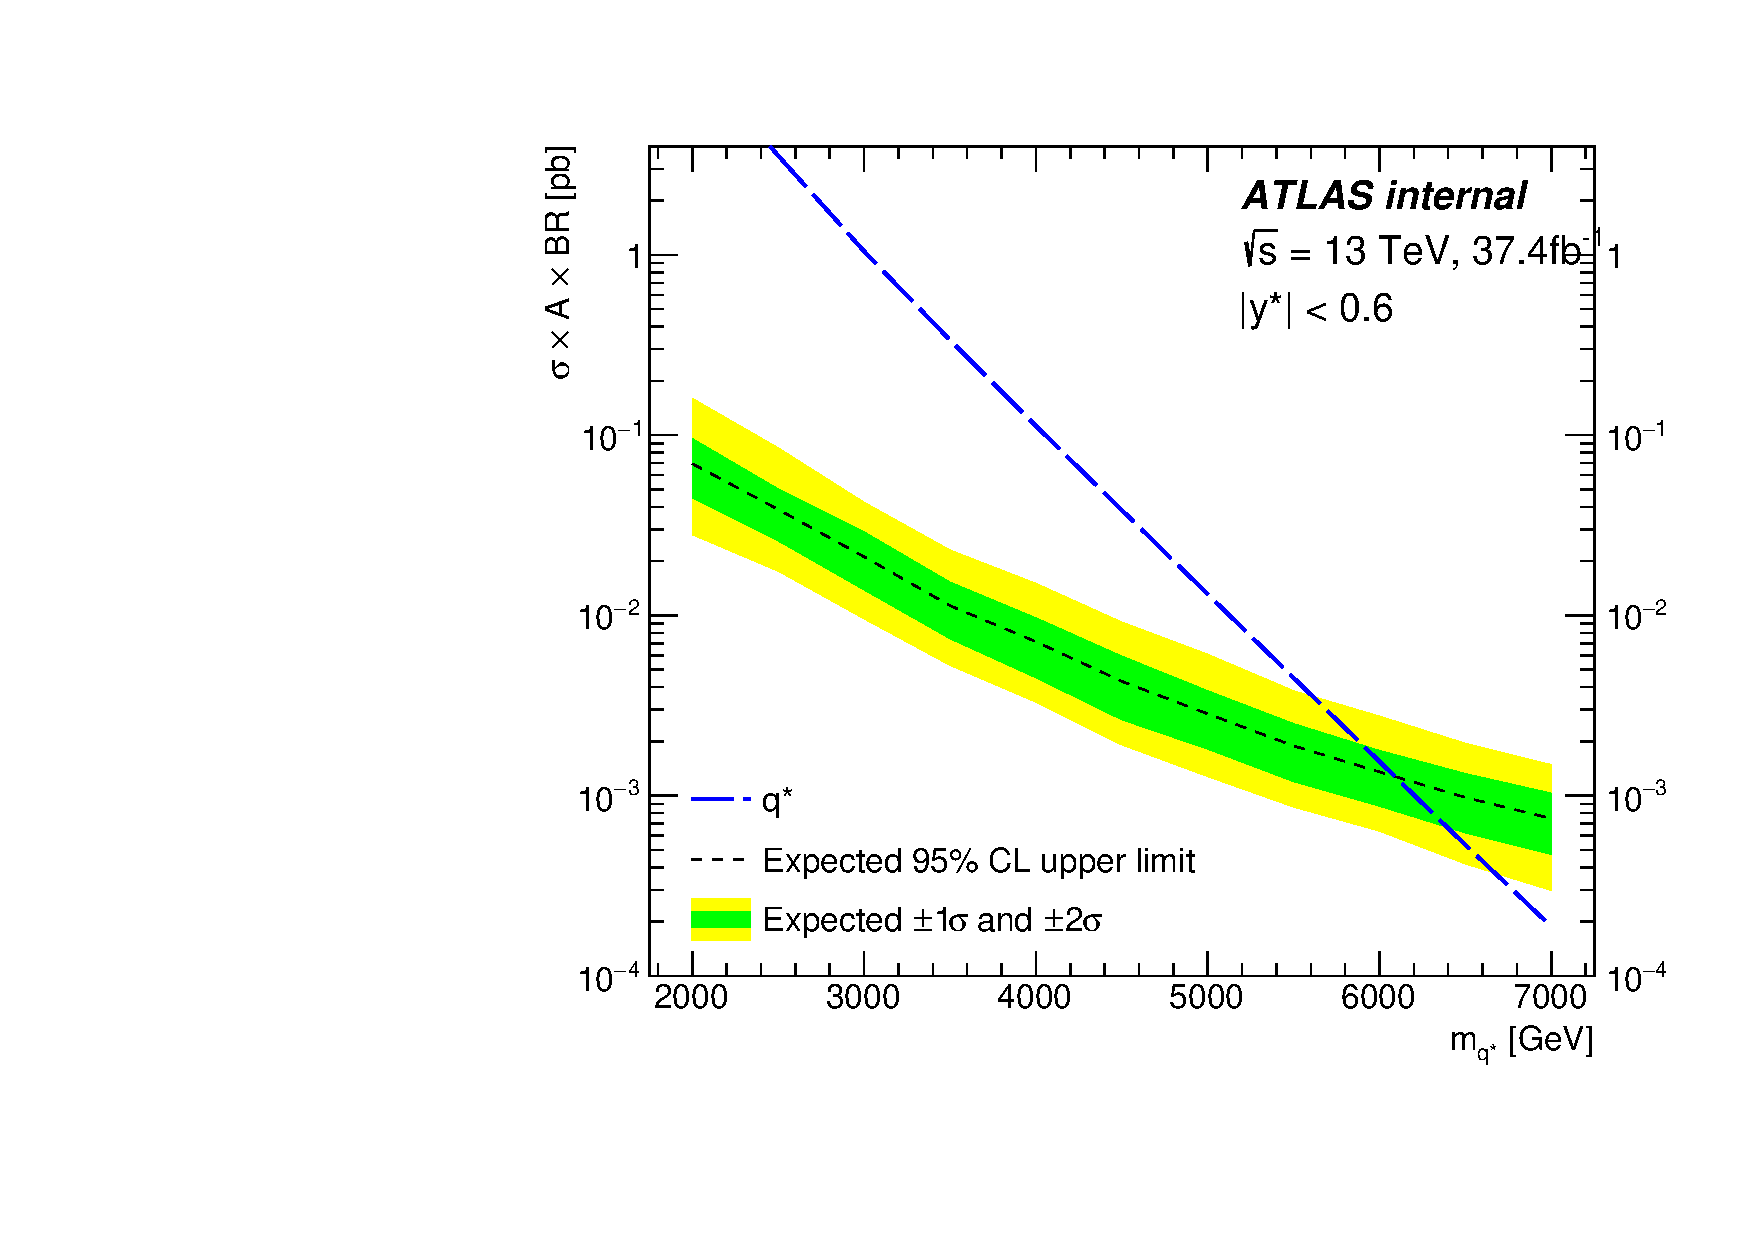
\includegraphics[width=0.475\textwidth] {figures/tagging/brazil-qStarMorphSingleJJUpdated.pdf}}
% \subfigure[\QQ\ \& \QG] {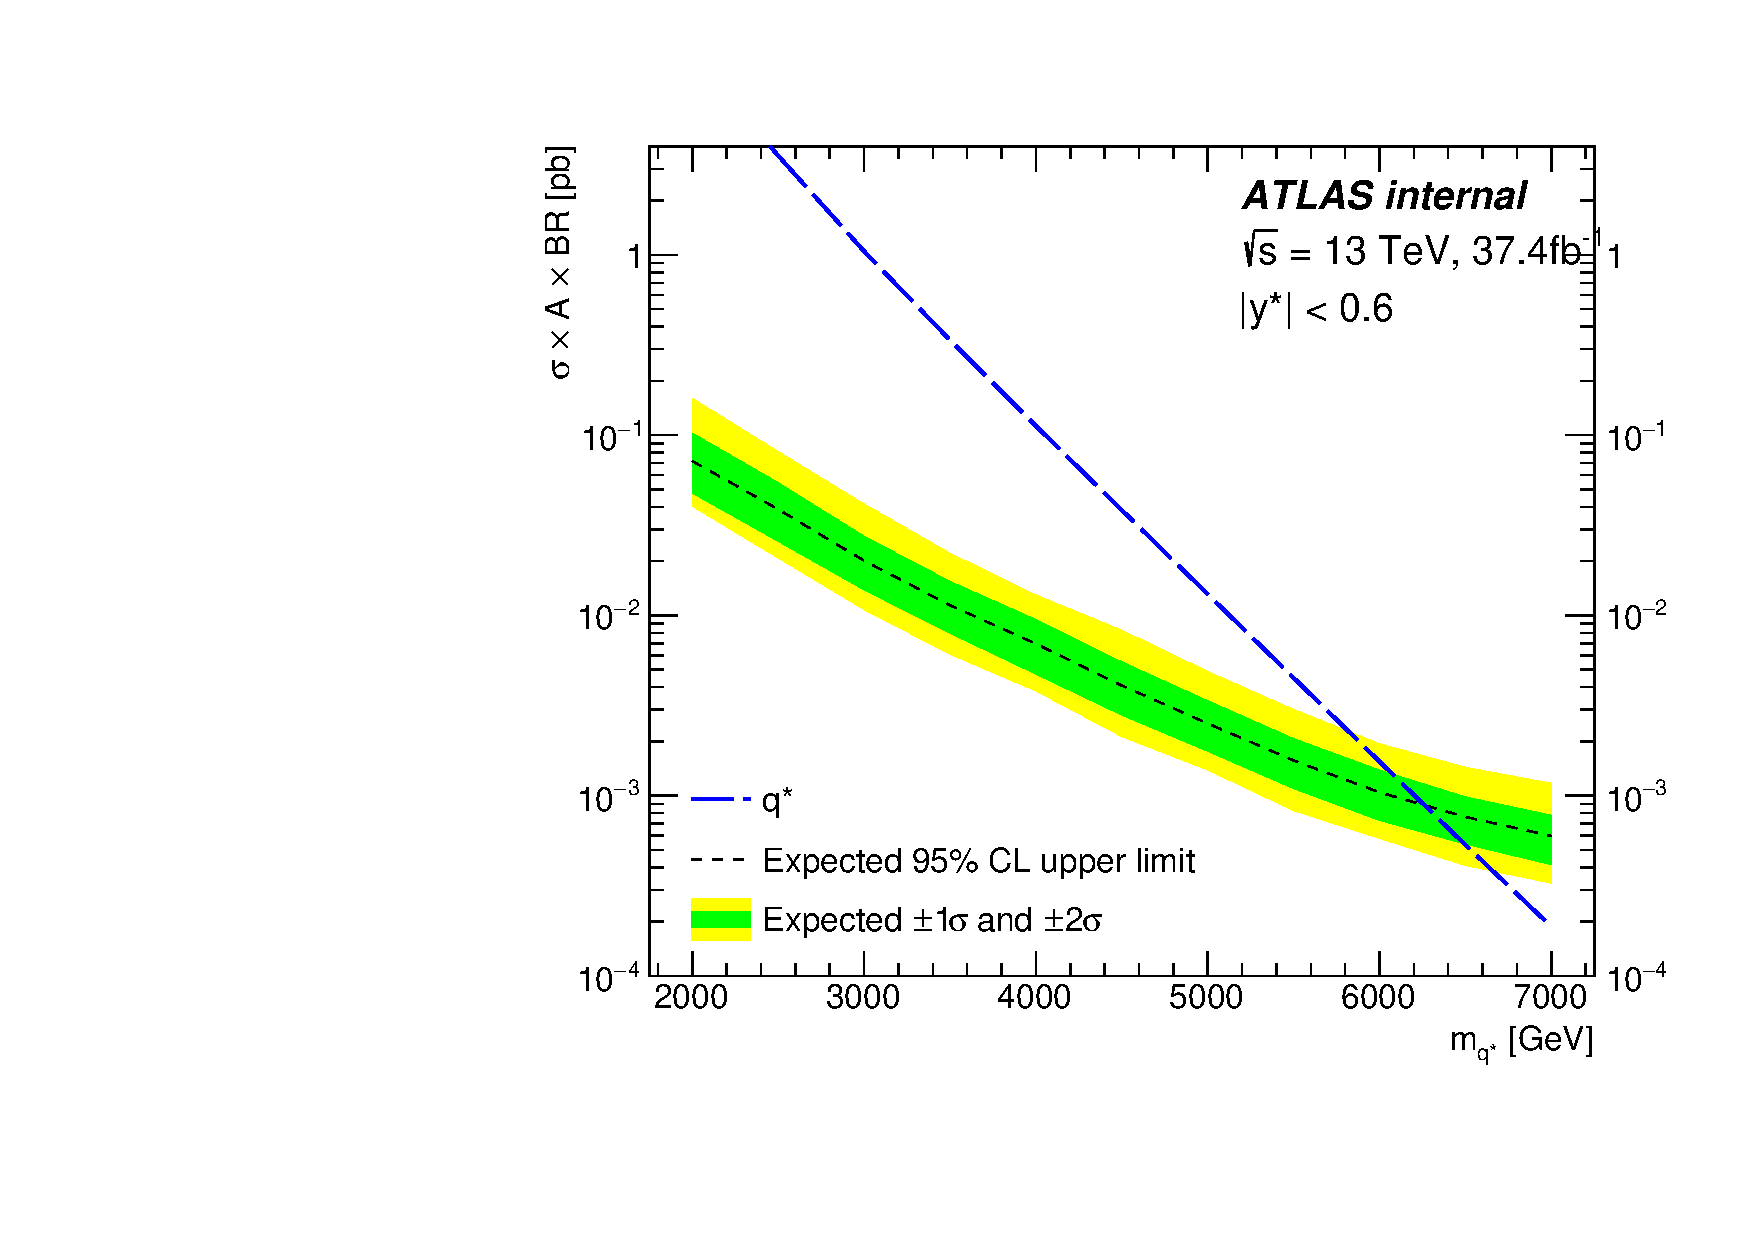
\includegraphics[width=0.475\textwidth] {figures/tagging/brazil-qStarMorphSingleCombinedUpdated.pdf}}
% \vspace*{-2mm}\\
% %
% \subfigure[\QQ] {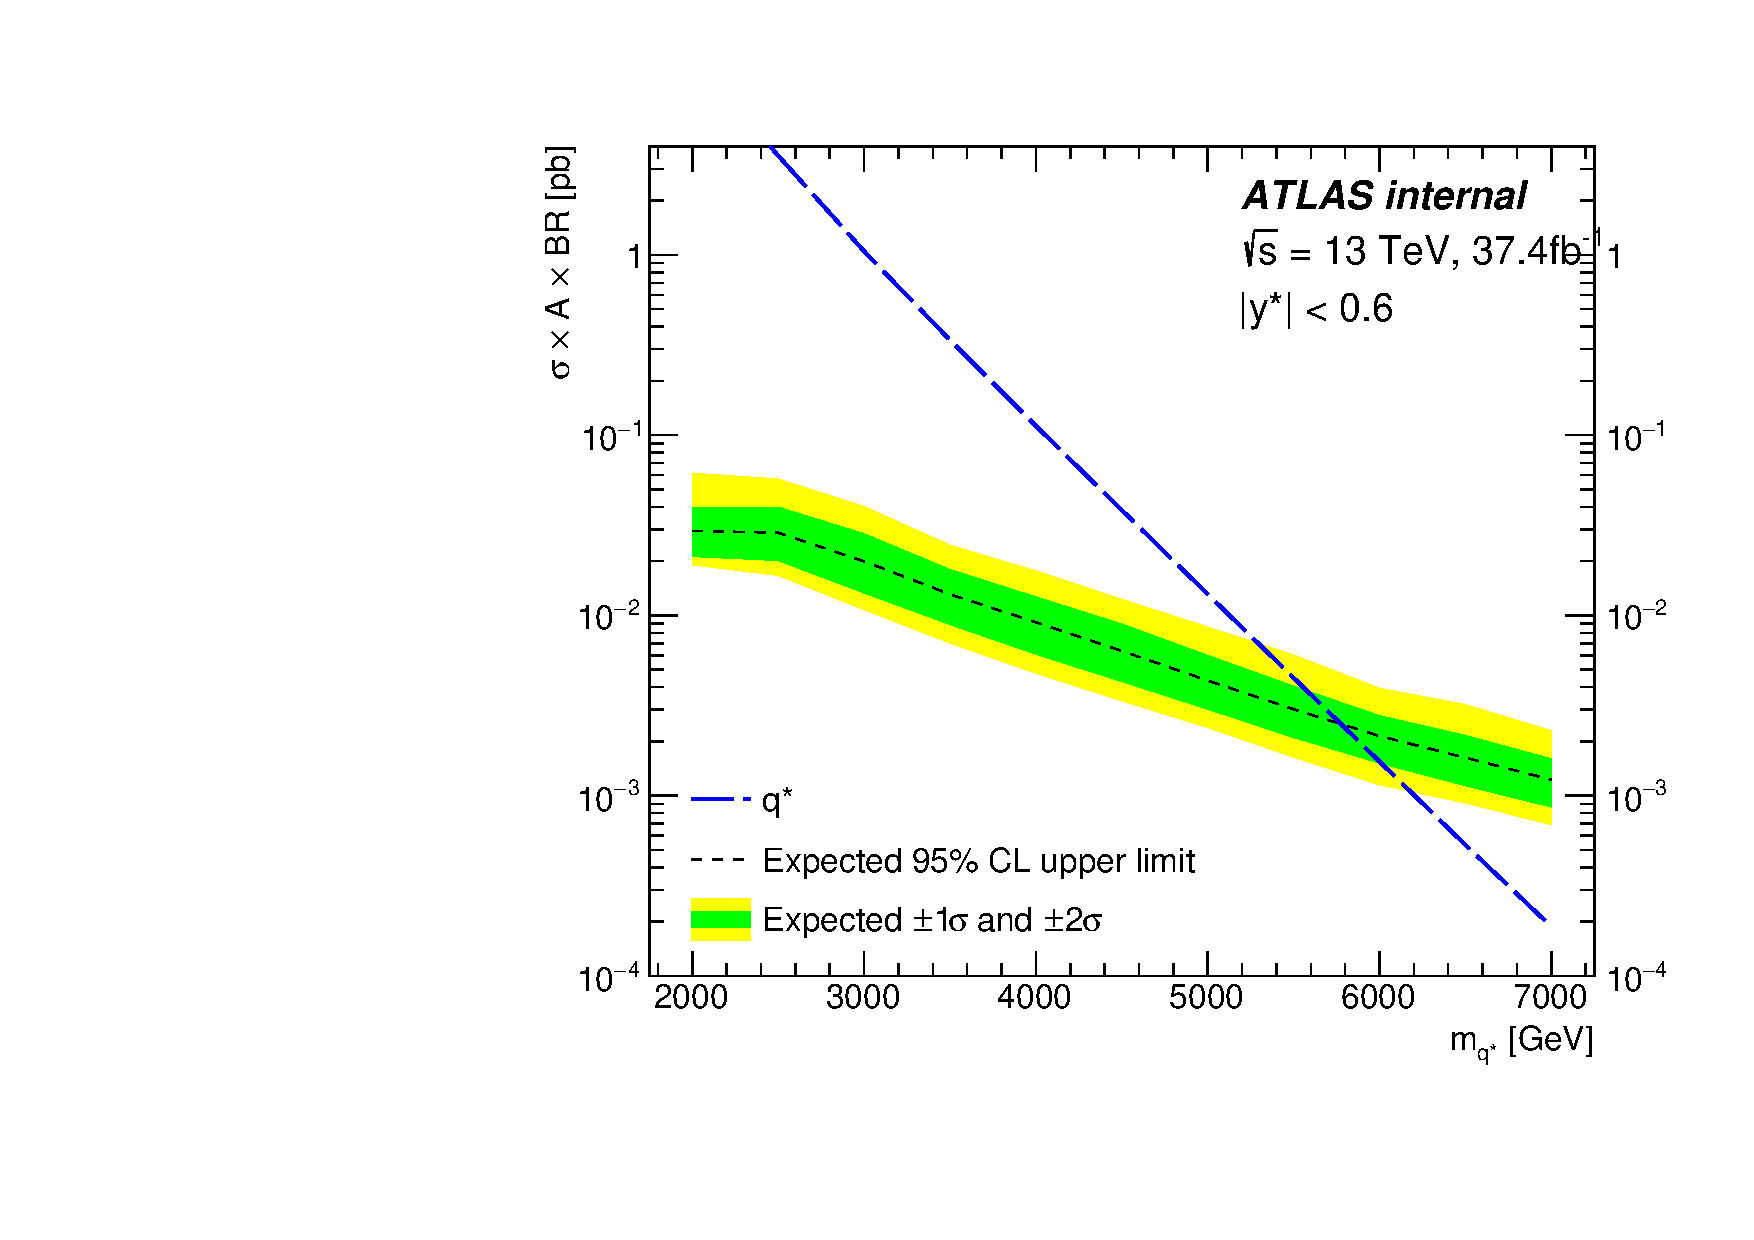
\includegraphics[width=0.475\textwidth] {figures/tagging/brazil-qStarMorphSingleQQUpdated}}
% \subfigure[\QG] {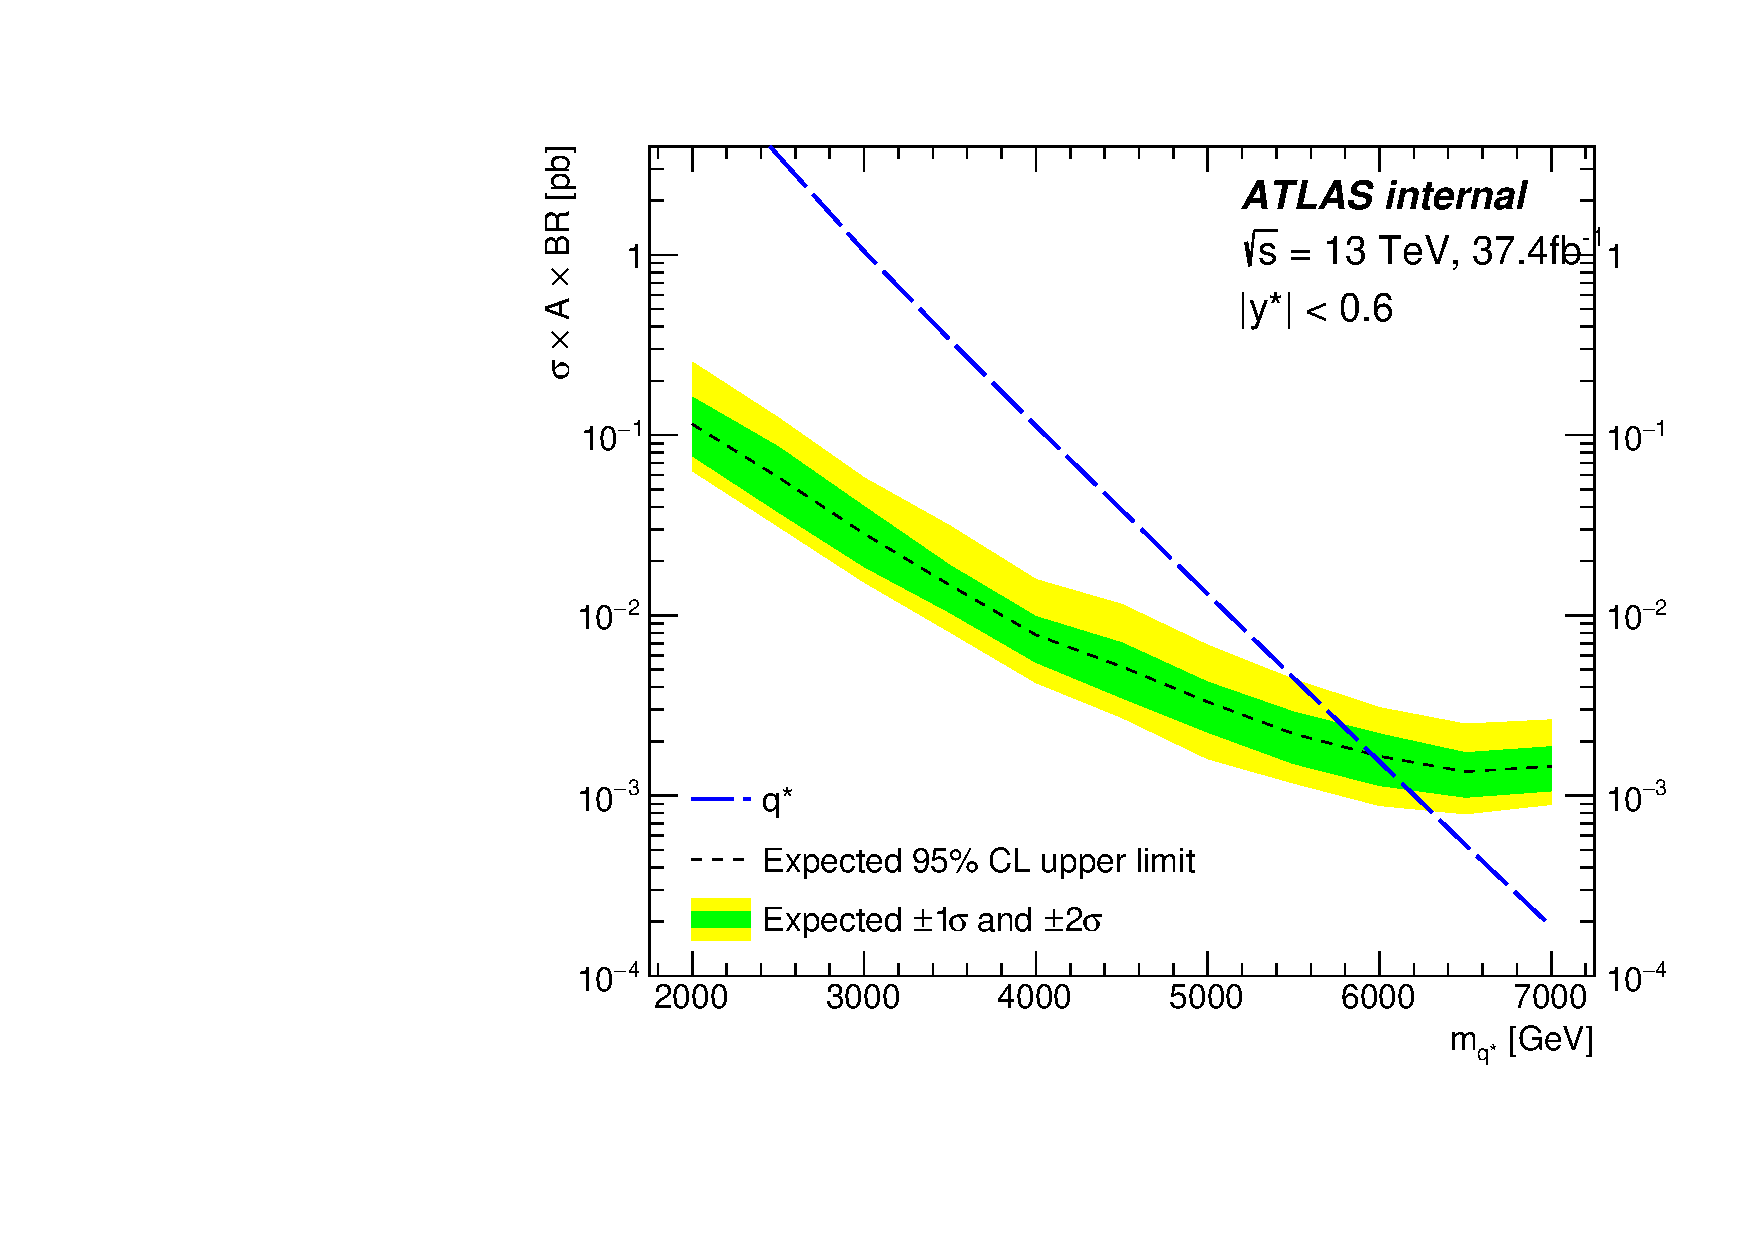
\includegraphics[width=0.475\textwidth] {figures/tagging/brazil-qStarMorphSingleQGUpdated}}
% \vspace*{-2mm}\\
% %
% \subfigure[\GG] {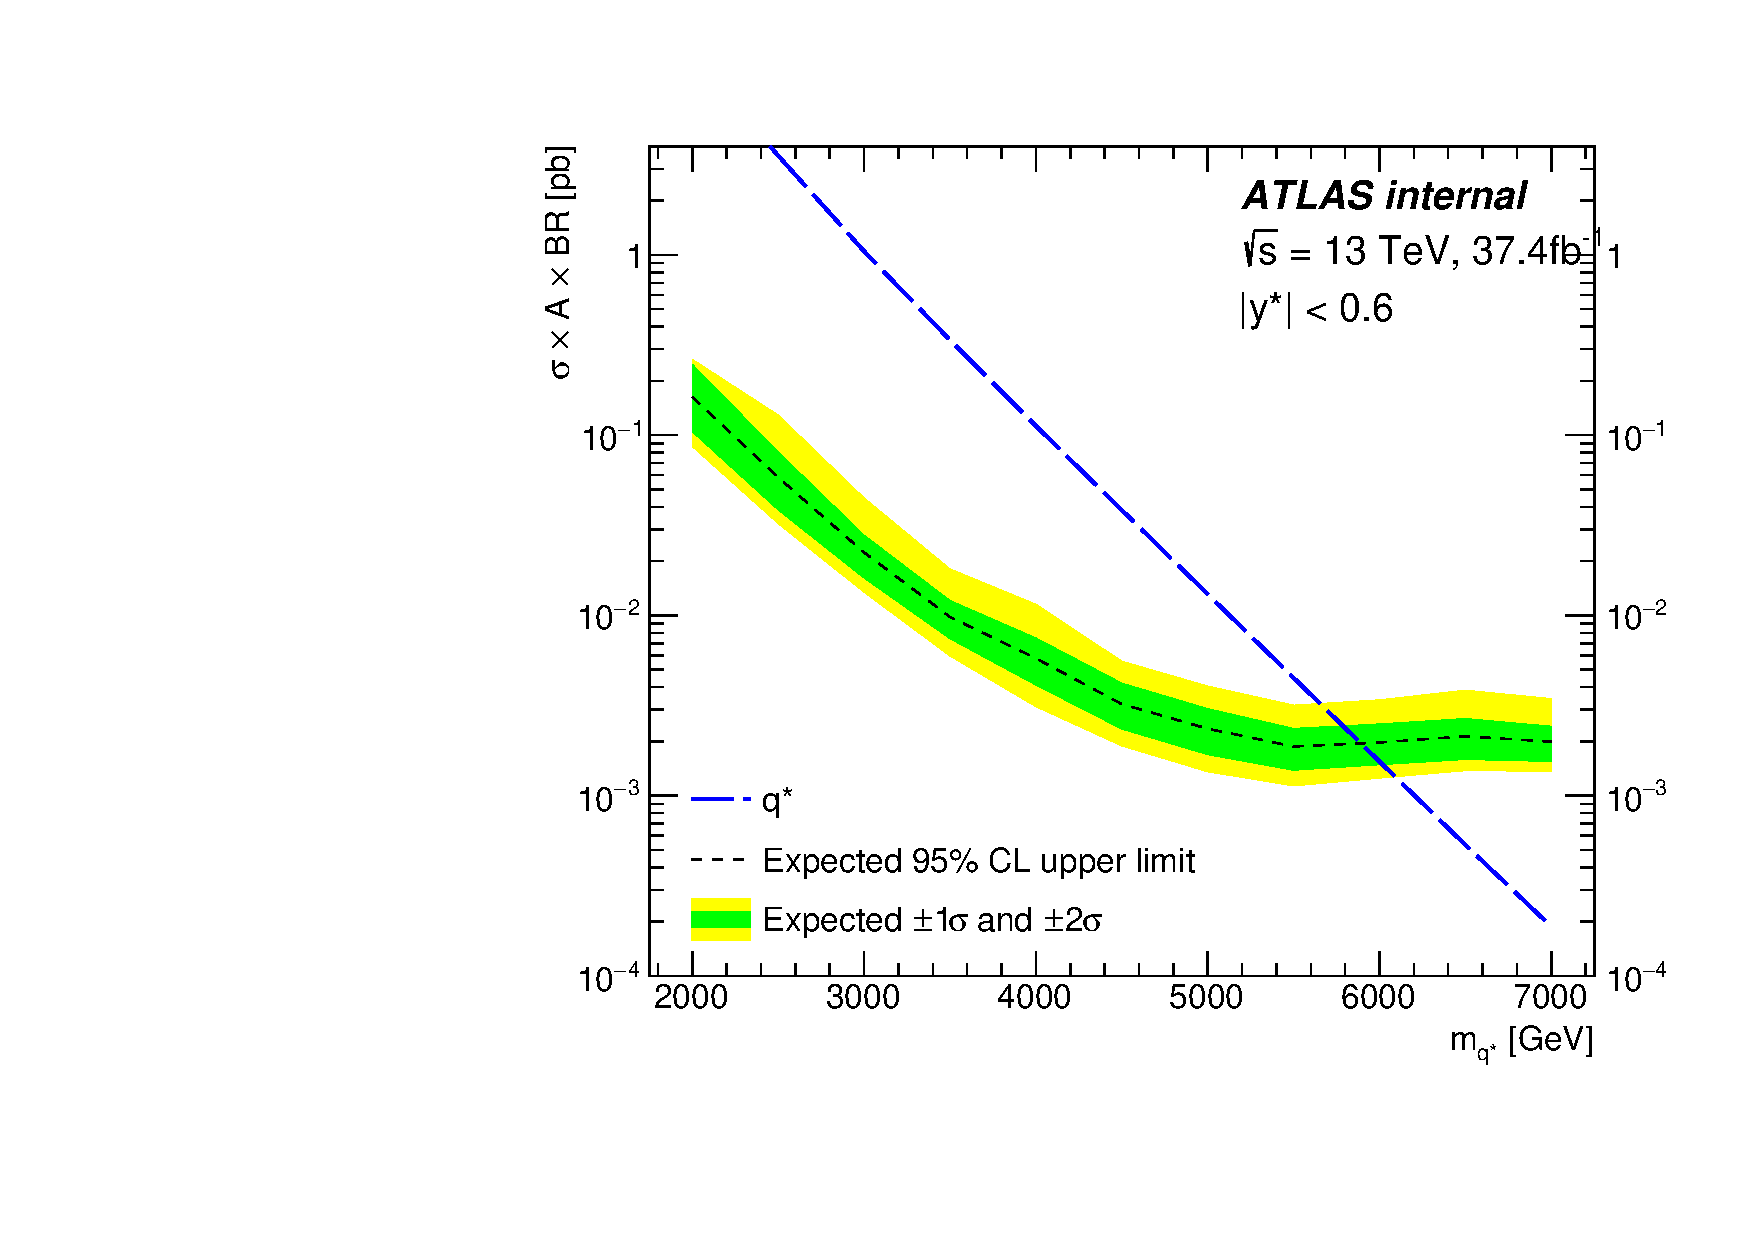
\includegraphics[width=0.475\textwidth] {figures/tagging/brazil-qStarMorphSingleGGUpdated}}
% \vspace*{-2mm}\\
% %
%
% \caption{Expected limits for a \qstar\ signal from  pseudo experiments for \integLumi\ for the 
% (a) \JJ\ resonant selection, (b) combined \QQ, \QG\ and \GG\ combined fit (c) \QQ\ sub-sample, (d) \QG\ sub-sample 
% and (e)  \GG\ sub-sample.
% \label{fig:toyMCExpectedLimitsqstar}}
%\end{figure}
%




